\section{Examples}

This section provides examples of using \pppx{} for various types of data processing.
The corresponding folder is `example/pppx/'.
Specifically, two RINEX files and some products are provided in "example/pppx/rinex/"
and "example/pppx/products/", respectively.
Basic information on the observation and product files can be found in
Tables~\ref{tab:data_for_example} and \ref{tab:products_for_example}, respectively.
Note that the VMF1 grid product is a file splicing the 00 h, 06 h, 12 h, and 18 h epochs
of the current day with the 00 h epoch of the next day.
By default, GPS and Galileo observations are used in each example,
except for the RTK example, which is GPS-only.

% The observations from stations ZIMM and ZIM2 on 2022-100 are used for demonstration.
% The following products are used for positioning:
 
\begin{table}[!hbt]
    \centering
    \caption{GNSS data used in examples.}
    \label{tab:data_for_example}
    \begin{tabular}{ll}
    \toprule
        Data & Description \\
    \midrule
        ZIM200CHE\_R\_20221000000\_01D\_30S\_MO.rnx & Rover station (GREC) \\
        ZIMM00CHE\_R\_20221000000\_01D\_30S\_MO.rnx & Reference station (G) \\
        ALGO00CAN\_R\_20221000000\_15M\_01S\_MO.rnx & High-rate data \\
    \bottomrule
    \end{tabular}
\end{table}


\begin{table}[!hbt]
    \centering
    \caption{Products used in examples.}
    \label{tab:products_for_example}
    \resizebox{\textwidth}{!}{
    \begin{tabular}{ll}
    \toprule
        Product & Description \\
    \midrule
        BRDC00IGS\_R\_20220010000\_01D\_MN.rnx & Broadcast ephemeris for multi-GNSS \\
        COD0MGXFIN\_20221000000\_01D\_05M\_ORB.SP3  & Precise orbit from CODE \\
        COD0MGXFIN\_20221000000\_01D\_30S\_CLK.CLK  & Precise clock from CODE \\
        COD0MGXFIN\_20221000000\_01D\_15M\_ATT.OBX  & Satellite attitude from CODE \\
        COD0MGXFIN\_20221000000\_01D\_01D\_OSB.BIA  & Satellite bias from CODE \\
        COD0MGXFIN\_20221000000\_03D\_12H\_ERP.ERP  & ERP from CODE \\
        codg1000.22i & GIM from CODE \\
        VMFG\_2022100 & spliced VMF1 grid from TU Vienna \\
    \bottomrule
    \end{tabular}}
\end{table}



\subsection{SPP: Single Point Positioning}

The \pppx{} software supports multi-GNSS SPP, including GPS, GLONASS, Galileo, BeiDou, and QZSS,
with broadcast ephemeris or precise satellite products.
Various tropospheric and ionospheric models are supported.
However, only the kinematic mode is currently supported, with either LSQ or FGO as the solver.
Note that LSQ- and FGO-based SPP are both epoch-wise solutions
(i.e., with no constraints between epochs); the only difference is that FGO uses the Huber loss
function (2 m threshold) to improve robustness.
Here, the LSQ solver is used, as the GNSS data in the examples are from geodetic-grade receivers.

Here, SPP solutions using the IF combination and single-frequency observations are demonstrated.
Both examples use broadcast ephemeris, which is the most common case for SPP users.
Specifically, the GMF model and the IF combination are used to correct tropospheric
and ionospheric delays for the IF solution, while the GMF model and a GIM product are used
for the single-frequency solution.
The other settings are kept at their defaults.
The corresponding configuration files can be found as "example/pppx/00\_spp\_if.ini"
and "example/pppx/01\_spp\_sf.ini", respectively.

% Note that the VMF1 model is used only to demonstrate how to use VMF1 grid, and GMF model should be sufficient for SPP. 

% 00\_spp\_if.ini
% \begin{minted}[frame=leftline]{ini}
% [model]
% trop = GMF
% iono = IF

% [product]
% src = brdc
% nav = BRDC_IGS_
% \end{minted}


The positioning results are shown in Figure~\ref{fig:example_spp}.
The single-frequency solution is better than the IF solution.
This is because the IF combination amplifies pseudorange noise by about a factor of three,
while the ionospheric delays can be well corrected with the GIM product for station ZIM2,
which is located at mid-latitude.

\begin{figure}
\centering
\begin{subfigure}{.35\paperwidth}
  \centering
  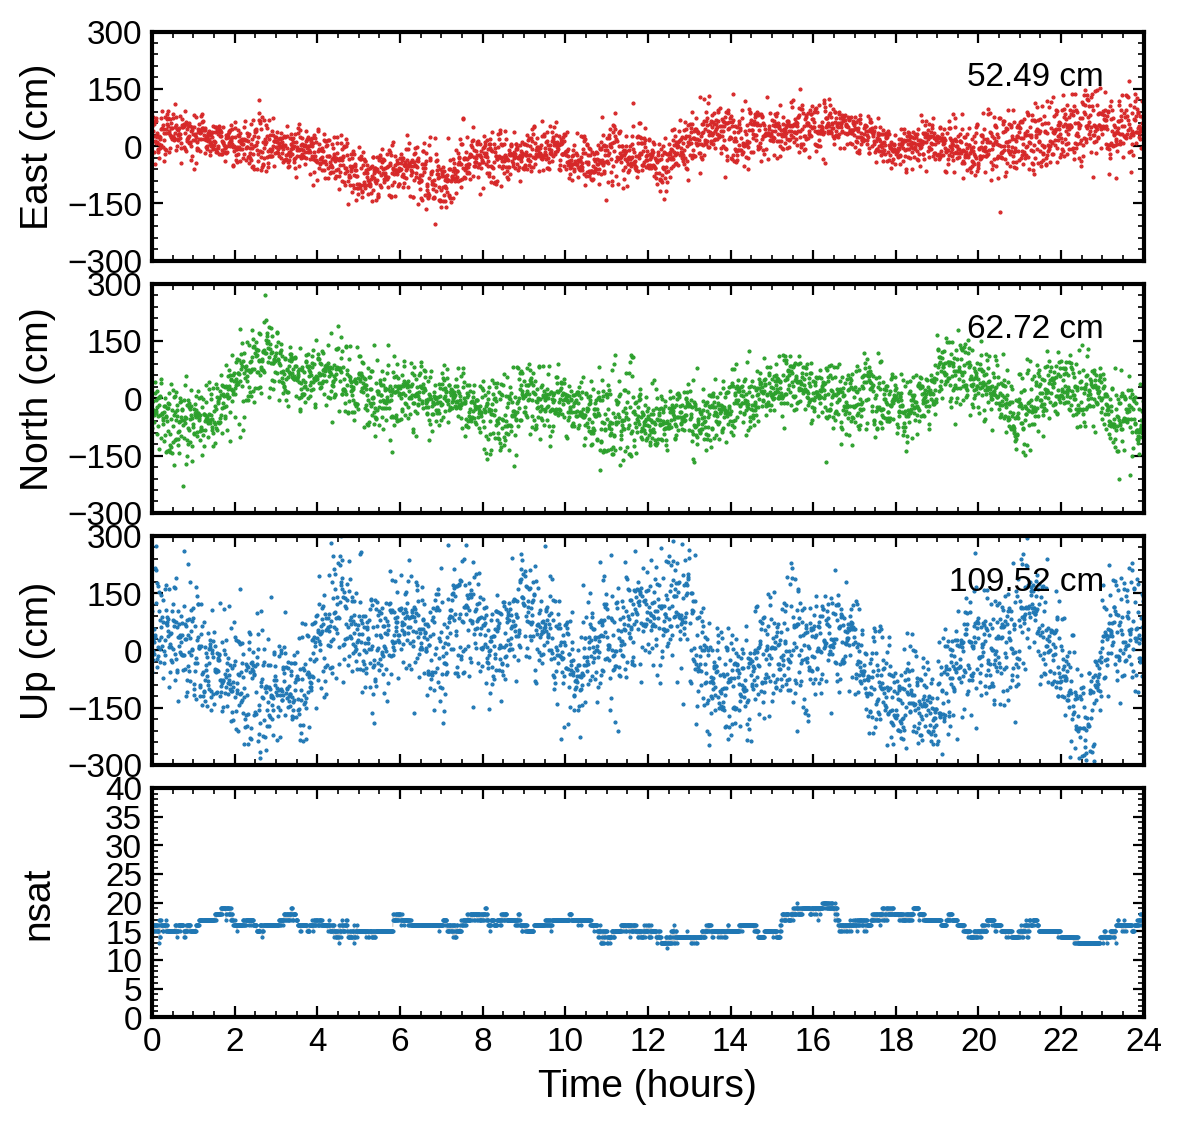
\includegraphics[width=1\linewidth]{figs/examples/spp_if.png}
  \caption{IF solution}
  \label{fig:example_spp_if}
\end{subfigure}%
\begin{subfigure}{.35\paperwidth}
  \centering
  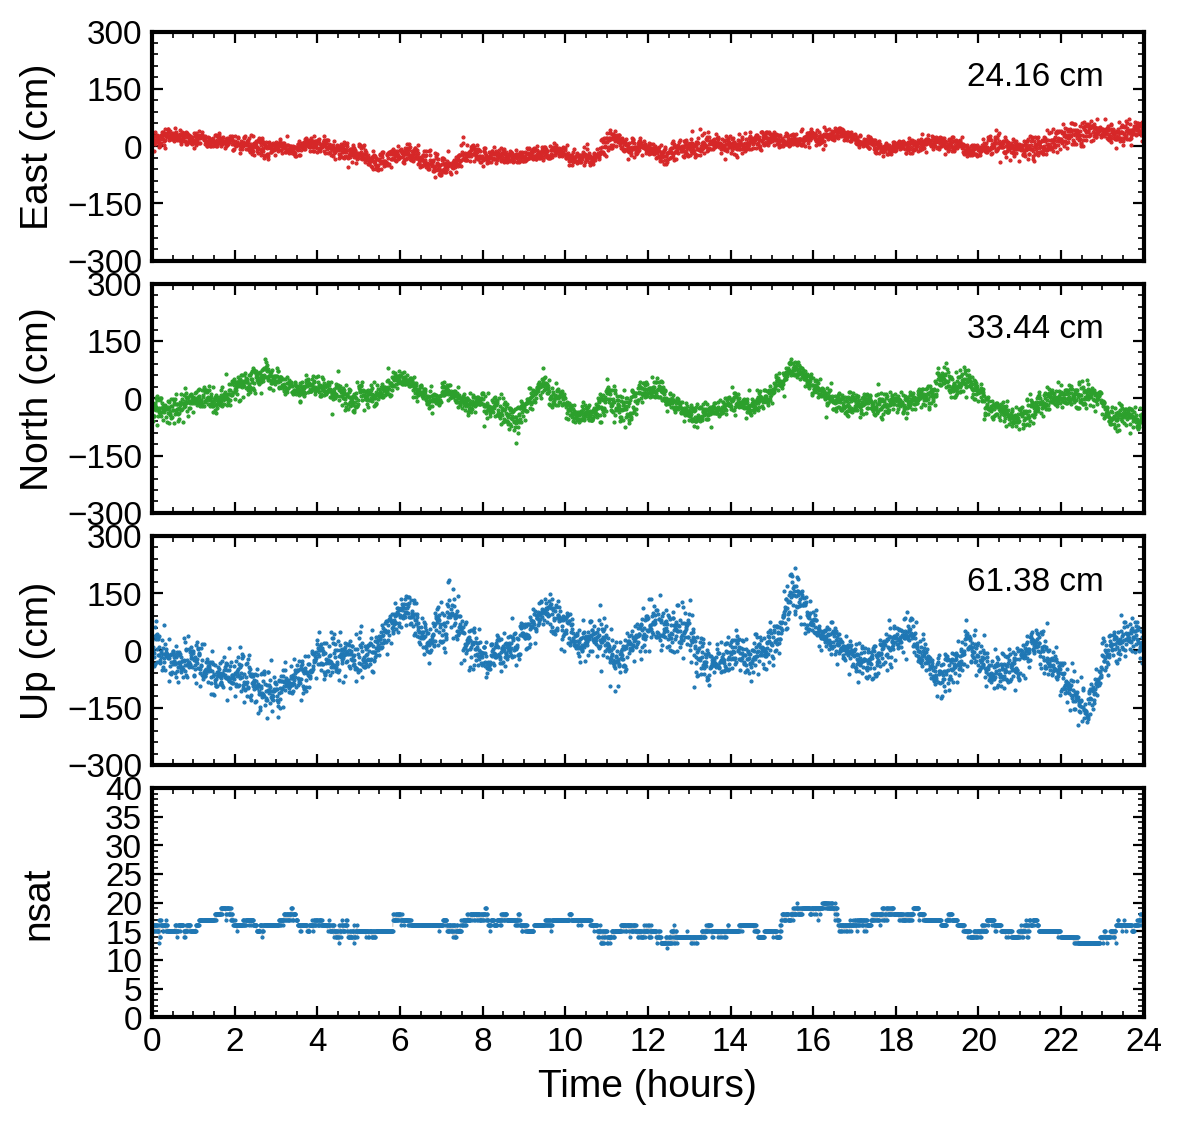
\includegraphics[width=1\linewidth]{figs/examples/spp_sf.png}
  \caption{SF solution}
  \label{fig:example_spp_sf}
\end{subfigure}
% \vspace{-2\baselineskip}
\caption{Positioning results of SPP solutions.}
\label{fig:example_spp}
\end{figure}



\subsection{PPP: Precise Point Positioning}

Here, PPP solutions are demonstrated with the Kalman filter or FGO as the solver.
The corresponding configuration files can be found as "example/pppx/02\_ppp\_ekf.ini"
and "example/pppx/03\_ppp\_fgo.ini", respectively.
The Kalman-filter-based solution simulates the real-time scenario
and outputs a forward-only solution.
The FGO-based solution is dedicated to post-processing and outputs a batch solution,
i.e., one without a convergence period.
In addition, FGO uses the Huber loss function to improve robustness,
with thresholds of 2 m and 0.02 m for pseudorange and carrier phase observations, respectively.

% \begin{enumerate}
%     \item PPP with EKF
%     \item PPP with FGO
%     \item PPP with brdc
% \end{enumerate}

The positioning results are shown in Figure~\ref{fig:example_ppp}.
There is no convergence period for the FGO-based solution,
whereas the EKF solution takes approximately 15 min to converge.
This is because FGO uses all the GNSS observations to form a single large LSQ problem
and solves all the parameters jointly, whereas EKF solves the parameters epoch by epoch.

\begin{figure}
\centering
\begin{subfigure}{.35\paperwidth}
  \centering
  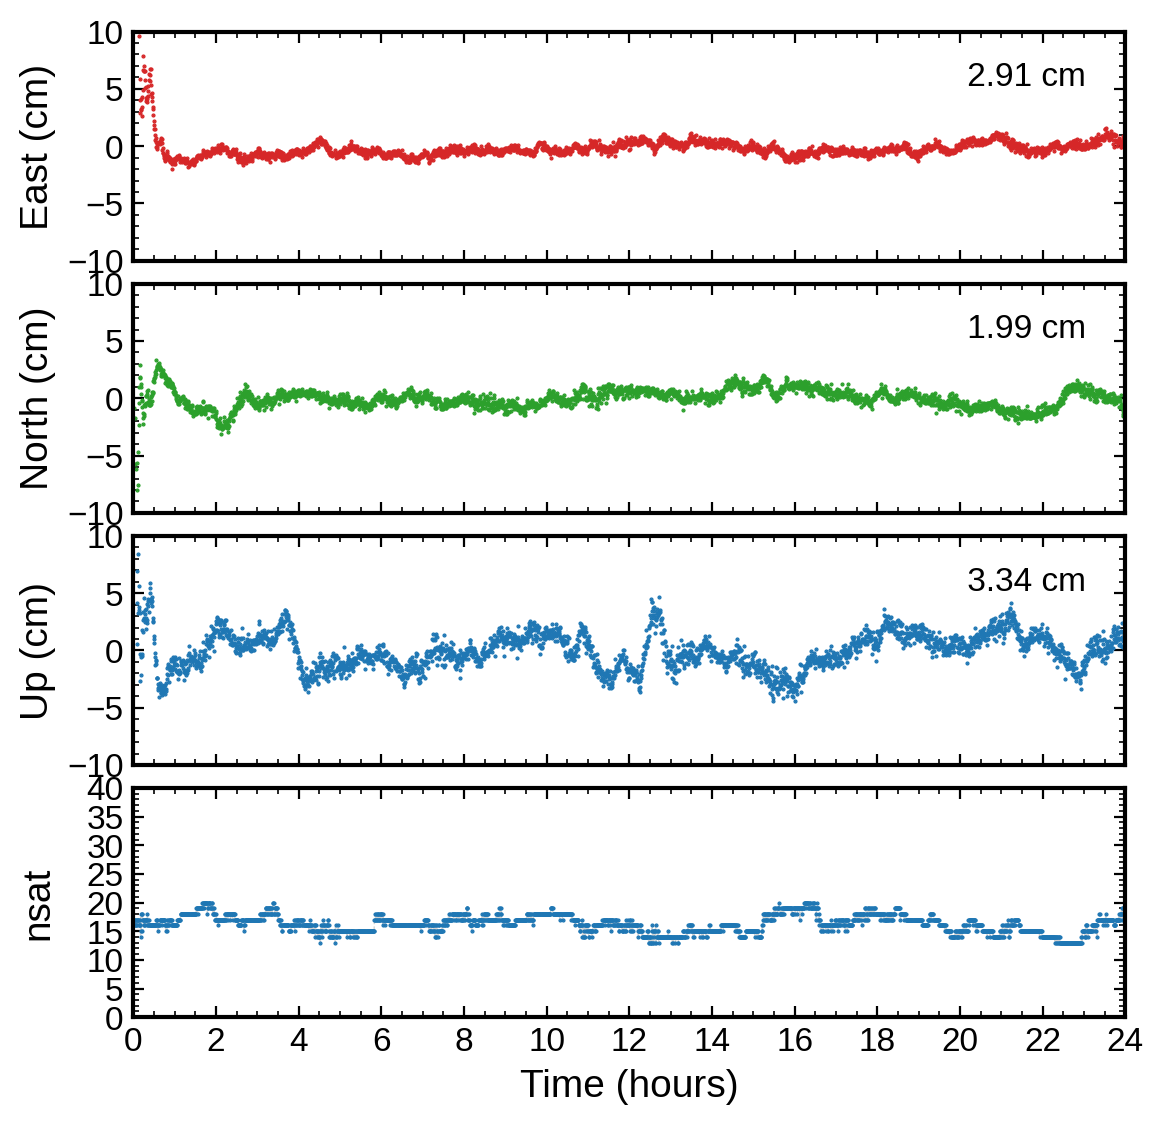
\includegraphics[width=1\linewidth]{figs/examples/ppp_ekf.png}
  \caption{EKF solution}
  \label{fig:example_ppp_ekf}
\end{subfigure}%
\begin{subfigure}{.35\paperwidth}
  \centering
  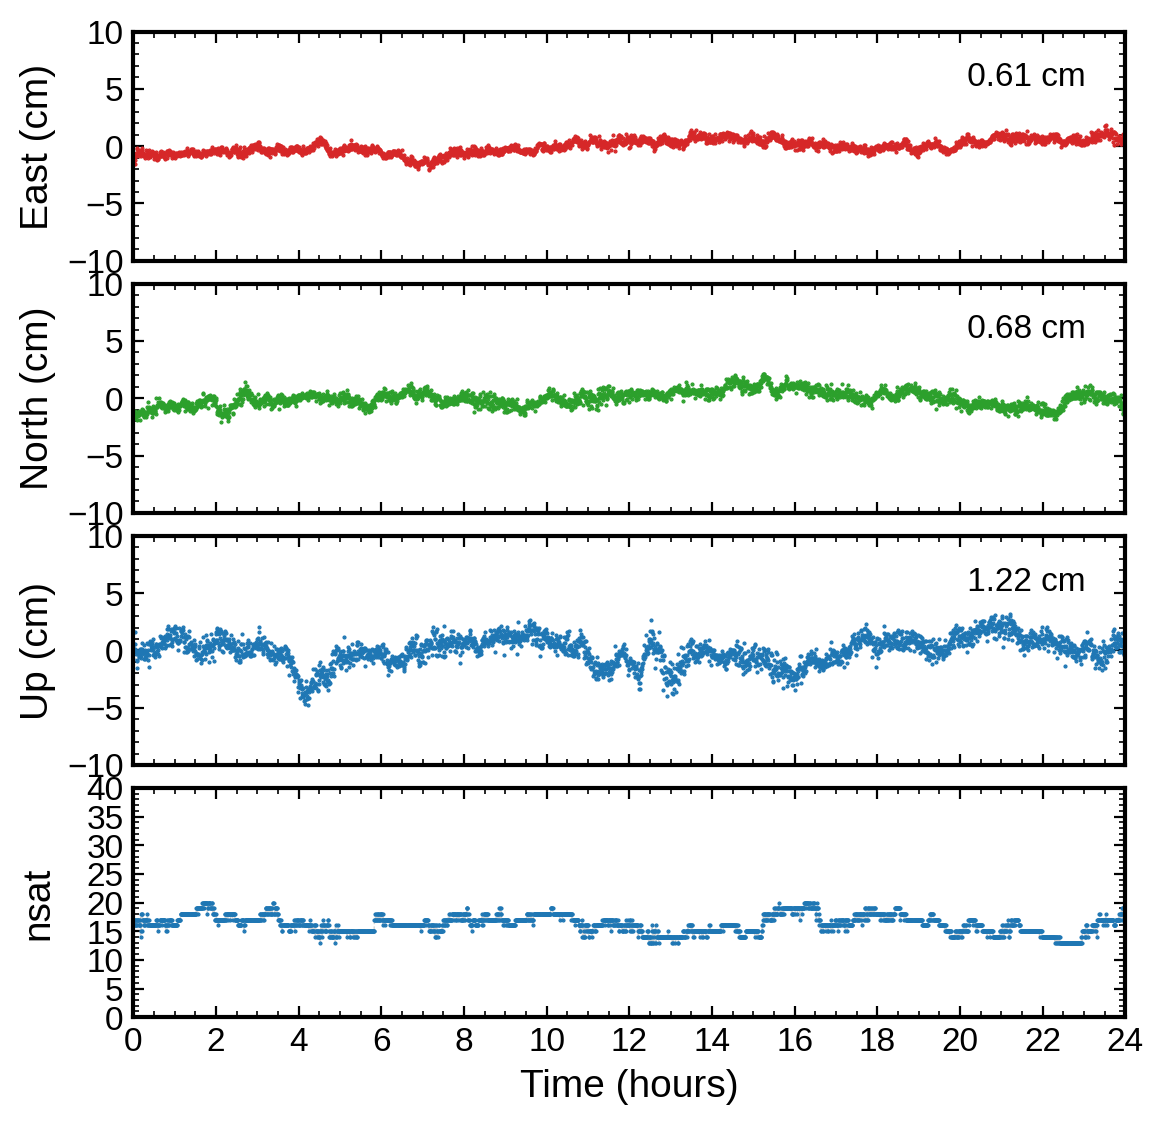
\includegraphics[width=1\linewidth]{figs/examples/ppp_fgo.png}
  \caption{FGO solution}
  \label{fig:example_ppp_fgo}
\end{subfigure}
% \vspace{-2\baselineskip}
\caption{Positioning results of PPP solutions.}
\label{fig:example_ppp}
\end{figure}



\subsection{RTK: Real-Time Kinematic}

The \pppx{} software only supports short baseline solutions.
Thus, "[model] trop" and "[model] iono" are always set to "none".
Both EKF and FGO are supported as solvers for RTK.
As before, the EKF solution simulates the real-time scenario and outputs a forward-only solution,
while the FGO solution is dedicated to post-processing
and outputs a batch solution without a convergence period.
The same Huber loss function as in PPP is adopted for FGO-based RTK processing.
Here, we show the RTK solution computed with EKF as an example.
The corresponding configuration file can be found as "example/pppx/06\_rtk.ini".

\begin{figure}[!hbt]
    \centering
    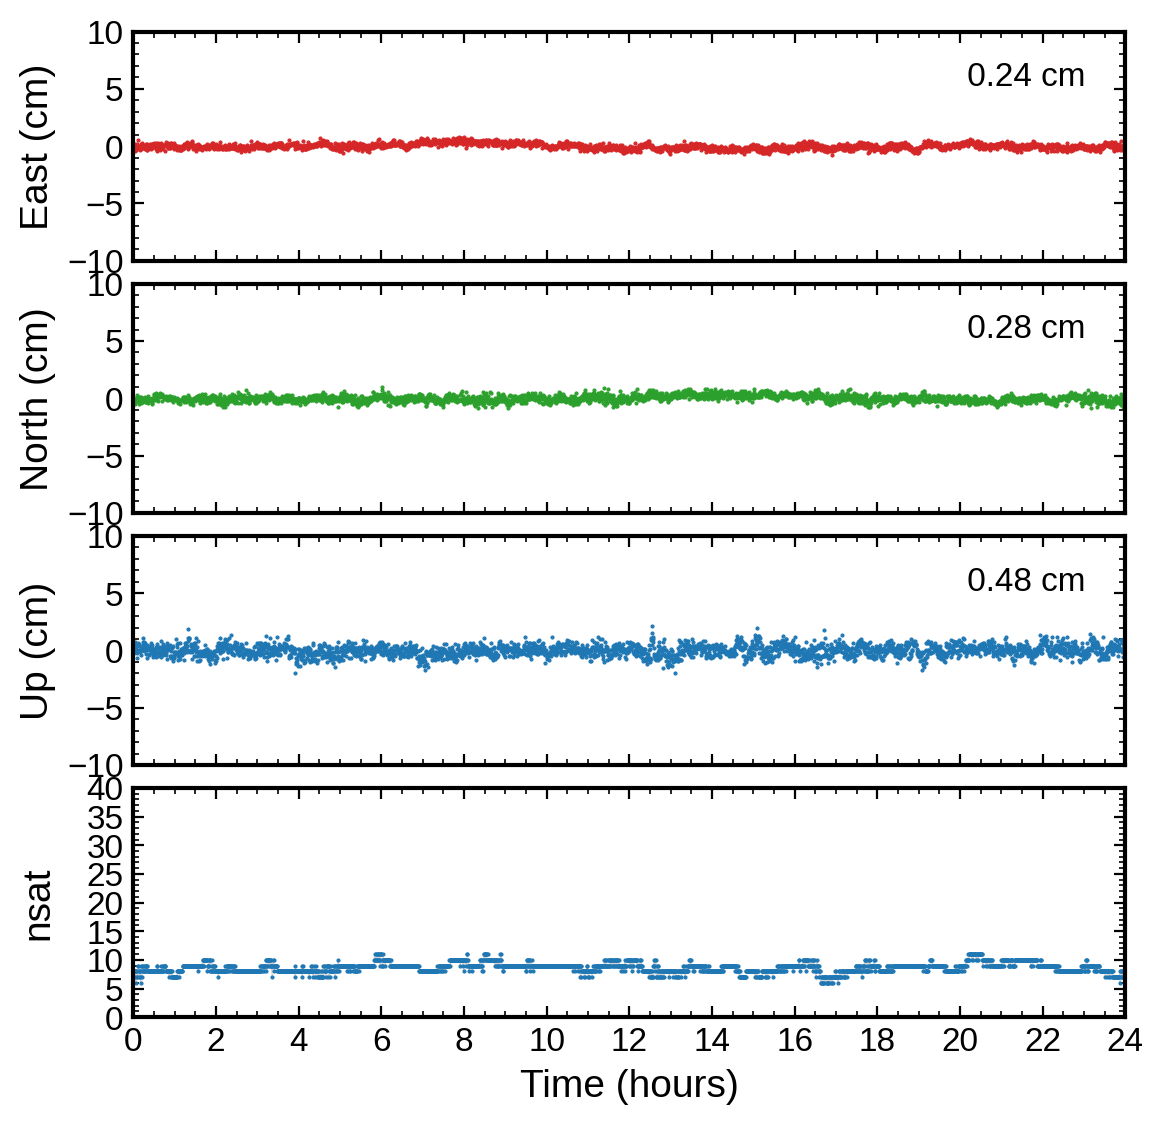
\includegraphics[width=.5\linewidth]{figs/examples/rtk.png}
    \caption{Positioning results of a short baseline solution between ZIM2 and ZIMM.}
    \label{fig:example_rtk}
    \vspace{-8pt}
\end{figure}

The positioning result is shown in Figure~\ref{fig:example_rtk}.
The precision is 0.24 cm, 0.28 cm, and 0.48 cm for the east, north, and up components, respectively.
These are typical precision values for short baseline solutions with resolved ambiguities.



\subsection{TDP: Time-Differenced Positioning}

TDP is useful for earthquake studies because it has no convergence time
and achieves high precision over a short time span.
Ambiguities are eliminated by time-differencing,
and the station displacements between adjacent epochs are estimated.
The displacements are then accumulated onto the initial station position,
and the absolute position for each epoch is written to the pos file.

An example is provided as "07\_tdp", where the 1-Hz GNSS data collected at the ALGO station
are processed with TDP.
Specifically, precise satellite products are used instead of broadcast ephemeris.
In this way, the drift in the positioning time series caused by error accumulation
becomes much smaller.
As ALGO is a static station, the ground truth displacement is zero.
The TDP positioning precisions over 15~min are 0.28~cm, 0.59~cm, and 0.93~cm
in the east, north, and up components, respectively.

\begin{figure}
    \centering
    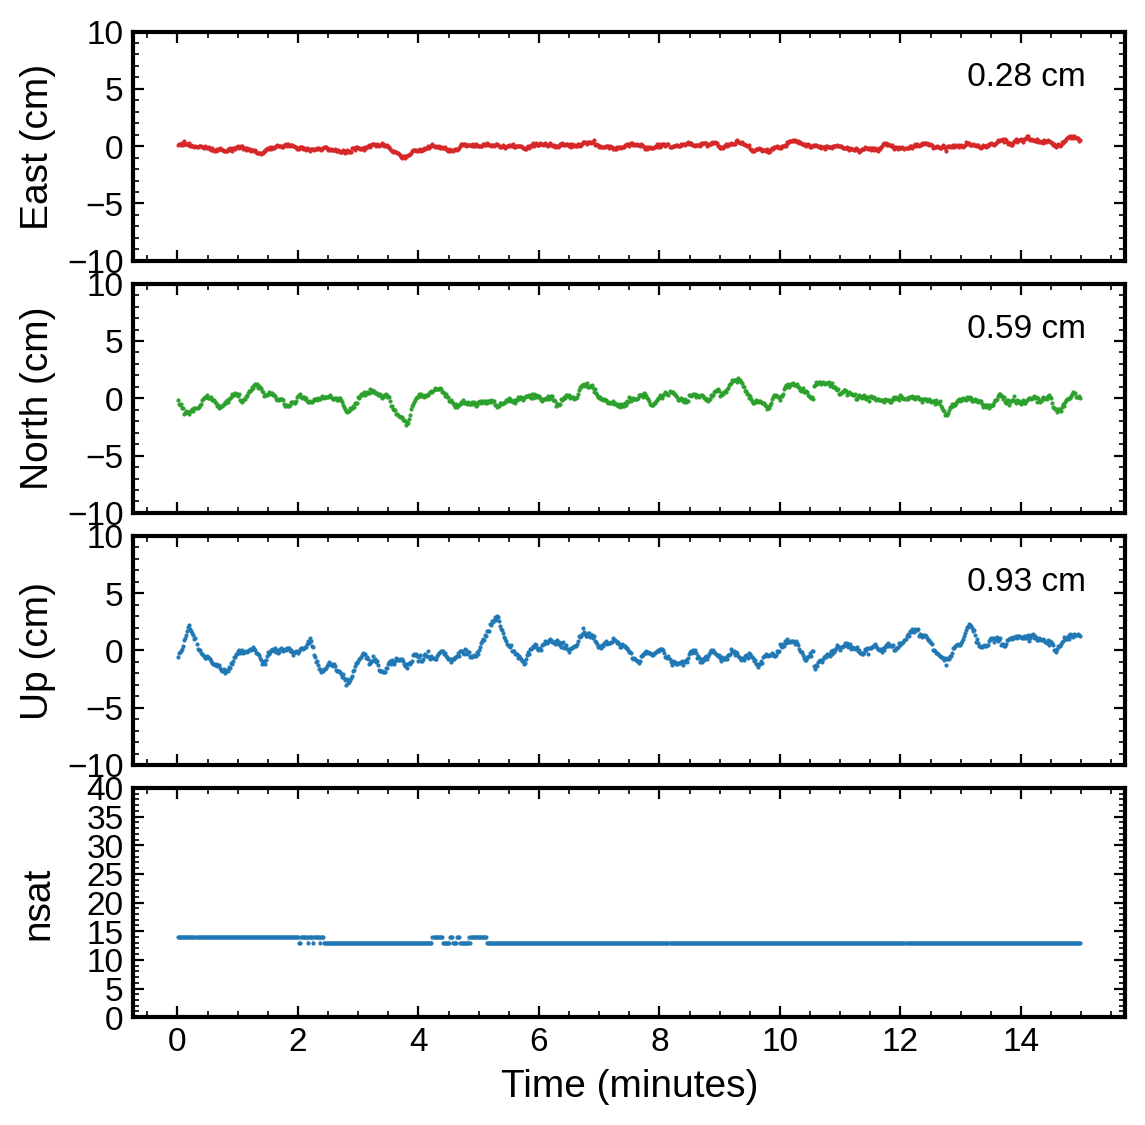
\includegraphics[width=.5\linewidth]{figs/examples/tdp.png}
    \caption{TDP positioning results for the ALGO station.}
    \label{fig:example_tdp}
    \vspace{-8pt}
\end{figure}